\documentclass[12pt,a4paper]{article}
\usepackage[english, science, large]{../template/ku-frontpage}
\usepackage{tabularx}
\usepackage{ltablex}
\usepackage{minted}
\setminted[text]{
frame=lines,
framesep=2mm,
baselinestretch=1.1,
fontsize=\footnotesize,
linenos,
breaklines}
\hypersetup{
    colorlinks=false,
    pdfborder={0 0 0},
}
\begin{document}

\title{ACS Theory Assignment 2}
\subtitle{}

\author{Kai Arne S. Myklebust, Silvan Adrian}
\date{Handed in: \today}
	
\maketitle
\tableofcontents

\section{Question 1: Concurrency Control Concepts}

\subsection{Task 1}
Following we have 2 schedules which are view equivalent. The first one is therefore view serializable.

\begin{table}[!htbp]
    \centering
    \begin{tabularx}{\textwidth}{l|l|l}
        \hline
        T1 & T2 & T3 \\ 
        \hline
        R(A) &  &  \\
             & W(A) & \\
             & commit & \\
        W(A) & & \\
        Commit & & \\
        		& & W(A) \\
        		& & Commit \\     
        \hline
    \end{tabularx}
\end{table}

\begin{table}[!htbp]
    \centering
    \begin{tabularx}{\textwidth}{l|l|l}
        \hline
        T1 & T2 & T3 \\ 
        \hline
        R(A) &  &  \\
        W(A) & & \\
        Commit & & \\        
             & W(A) & \\
             & commit & \\
        		& & W(A) \\
        		& & Commit \\     
        \hline
    \end{tabularx}
\end{table}

And the precedence graph of the first schedule shows that there is a cycle, which means it's not conflict serializable.
\begin{figure}
	\center
	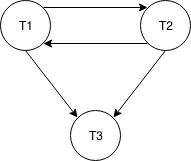
\includegraphics{img/Q1-task1}
	\caption{Precedence Graph for shedule}
\end{figure}

\subsection{Task 2}


\subsection{Task 3}


\subsection{Task 4}

\section{Question 2: Recovery Concepts}
\subsection{Task 1}
We do not need a redo scheme, because all changes of committed transactions are guaranteed to have been written to disk at commit time.
We also don't need the undo scheme, because the changes of those aborted transactions have not been written to disk.

\subsection{Task 2}
The difference of stable storage and non-volatile storage is that stable storage is implemented by maintaining multiple copies of information on non-volatile storage.
Access time on non-volatile storage is therefore much faster than on stable storage.

Non-volatile storage is guaranteed to survive crashes but can be subject to media failures, while stable storage is guaranteed to survive both.


\subsection{Task 3}
The log tail needs to be forced to stable storage in following 2 situations:
\begin{itemize}
	\item When a transaction is committed
	\item After modifying of pages	
\end{itemize}

For the first situation, when a transaction is committed it has be ensured that the record of changes have been written in the log before it's written to disk.
This way we know what changes have been done even after a crash.

For the second situation, when a page gets modified we have to know that there has been a change without committing so that we are able to undo the not committed changes. 

For both situations the durability is sufficient because we are able to undo modifications and ensure that all committed transactions survive a crash.

\section{Question 3: More Concurrency Control}
\subsection{Task 1}
There are no locks waiting on each other. And after commit all exclusive locks get released and we have in transaction Ta and Tc only a shared lock on Z.
% shedule 1 S2PL
\begin{table}[!htbp]
    \centering
    \begin{tabularx}{\textwidth}{l|l|l}
        \hline
        Ta & Tb & Tc \\ 
        \hline
        S(Z) &  &  \\
        R(Z) &  &  \\
             & S(Y) & \\
             & R(Y) & \\
             & X(Y) & \\             
             & W(Y) & \\
             &  & S(Z)\\             
        	 &  & R(Z)\\
       		& C & \\        	 
       		& Release(Y) & \\
        	& & X(Y) \\       		
        	& & W(Y) \\
        	& & C \\ 
			& & Release(Z,Y) \\
		X(Y) & &  \\  
        W(Y) & &  \\   
        C & &  \\   
        Release(Z,Y) & &  \\ 
        \hline
    \end{tabularx}
\end{table}
\subsection{Task 2}
Locks are not waiting on each other and they get released on time before an other transaction wants to get a lock on the same object.
% 2PL
\begin{table}[!htbp]
    \centering
    \begin{tabularx}{\textwidth}{l|l|l}
        \hline
        Ta & Tb & Tc \\ 
        \hline
        S(Z) &  &  \\
        R(Z) &  &  \\
        Release(Z) &  &  \\        
             & S(Y) & \\
             & R(Y) & \\
             & X(Y) & \\             
             & W(Y) & \\
			 & Release(Y) & \\
             &  & S(Z)\\             
        	 &  & R(Z)\\
			& & Release(Z) \\        	 
       		& C & \\        	 
        	& & X(Y) \\       		
        	& & W(Y) \\
			& & Release(Y) \\
        	& & C \\ 
		X(Y) & &  \\  
        W(Y) & &  \\ 
		Release(Y) & &  \\ 
        C & &  \\   
        \hline
    \end{tabularx}
\end{table}
\subsection{Task 3}
No not possible, since we acquire an exclusive lock on \texttt{Y} in \texttt{Ta} and afterwords try to get an other exclusive lock on \texttt{Y} in \texttt{Tb} which is not allowed in \texttt{CS2PL}.
\begin{table}[!htbp]
    \centering
    \begin{tabularx}{\textwidth}{l|l|l}
        \hline
        Ta & Tb & Tc \\ 
        \hline
        S(X) &  &  \\
        X(Y) &  &  \\
        R(X) &  &  \\
        	 & X(Z) &  \\
   			 & X(Y) - Not possible, abort &  \\          
        \hline
    \end{tabularx}
\end{table}

\subsection{Task 4}
We decided that \texttt{Tb} will be the first transaction, \texttt{Tc} the second and \texttt{Ta} the last.
\begin{minted}{text}
Tb: RS(Tb) = {Z,Y}, WS(Tb) = {Z,Y},
Tb completes before Tc starts.
Tc: RS(Tc) = {Z}, WS(Tc) = {Z},
Tc completes before Ta starts with its write phase.
Ta: RS(Ta) = {X}, WS(Ta) = {Y}.
\end{minted}

\begin{itemize}
	\item \texttt{Tb} completes before \texttt{Tc} starts, so there weren't any conflicts with other transactions while validation.	
	\item \texttt{Tc} completes before \texttt{Ta} starts with its write phase and the intersection of the write set from \texttt{Tc} and read set from \texttt{Ta} is empty.
	\item So according to the validation phase in \texttt{KROCC} the three transactions have no conflicts so this schedule could be generated by \texttt{KROCC}.
\end{itemize}

\section{Question 4: ARIES}

\subsection{Task 1}
Following 2 tables are the transaction table and the dirty page table after the analysis phase of ARIES.

Transaction table:
\begin{table}[!htbp]
    \centering
    \begin{tabularx}{\textwidth}{l|l|l}
        \hline
        TransID & Status & LastLSN \\ 
        \hline
        T1 & Active & 4 \\
        T2 & Active & 9 \\         
        \hline
    \end{tabularx}
\end{table}

Dirty Page table:
\begin{table}[!htbp]
    \centering
    \begin{tabularx}{\textwidth}{l|l}
        \hline
        PageId & RecLSN \\ 
        \hline
        P2 & 3 \\
        P1 & 4 \\
        P5 & 5 \\
        P3 & 6 \\         
        \hline
    \end{tabularx}
\end{table}

\subsection{Task 2}
The winner set of transactions is: \{T3\} because it was able to commit and finish.
The loser set of transactions is: \{T1,T2\} because they weren't able to finish and were still active while the crash occured.

\subsection{Task 3}
The redo phase start with log record with the smallest \texttt{recLSN} in the dirty page table, in this case it would be \texttt{LSN 3}.
The undo phase goes through all loser transactions and ends at the oldest \texttt{LSN}, in this case it would be \texttt{LSN 3}.
\subsection{Task 4}
To get the set of log records to be redone we start by taking the smallest \texttt{LSN} from the dirty page table. And add the modifications with higher \texttt{LSNs} then the smallest \texttt{LSN} from the dirty page table to the set as well.

So we get the following set: \{3,4,5,6,8,9\}
\subsection{Task 5}
To get the set of records undone, we have to get all the updates from the loser transactions starting from the newest one.
We would get the following set: \{9,8,5,4,3\}
\subsection{Task 6}
The following table is only the appended log entries after the crash.
\begin{table}[!htbp]
    \centering
    \begin{tabularx}{\textwidth}{l|l|l|l|l|l}
        \hline
        LSN & LAST\_LSN & TRAN\_ID & TYPE & undoNextLSN & PAGE\_ID \\ 
        \hline
        11 & 9  & T2 & ABORT & & \\
      	12 & 4  & T1 & ABORT & & \\      
      	13 & 11 & T2 & CLR: Undo LSN 9 &  8 & \\
      	14 & 13 & T2 & CLR: Undo LSN 8 & 5 & \\
      	15 & 14 & T2 & CLR: Undo LSN 5 & - & \\
      	16 & 15 & T2 & end & & \\
      	17 & 12 & T1 & CLR: Undo LSN 4 & 3 & \\
      	18 & 17 & T1 & CLR: Undo LSN 3 & - & \\
      	19 & 18 & T1 & end & & \\     
        \hline
    \end{tabularx}
\end{table}

\section{Question 5: More ARIES}
\subsection{Task 1}
\begin{itemize}
	\item A has the value 5, since we are currently undoing 7 and the previous \texttt{LSN} in T2 is 5	
	\item B has the value 4, since we are currently undoing 9 and the previous \texttt{LSN} in T1 is 4
	\item C has the value 3, since we are currently undoing 4 and the previous \texttt{LSN} in T1 is 3
	\item D has the value NULL, since we are currently undoing 5 and the previous \texttt{LSN} in T2 is NULL
	\item E has the value NULL, since we are currently undoing 3 and the previous \texttt{LSN} in T1 is NULL
\end{itemize}

\subsection{Task 2}
Since we don't have a new checkpoint yet, we have to start over from \texttt{LSN 3} for the dirty page table.
T1 is undone and ended, and T4 is committed and ended, so they are not in the transaction table.
So that we ended up on the following 2 tables:

Transaction table:
\begin{table}[!htbp]
    \centering
    \begin{tabularx}{\textwidth}{l|l|l}
        \hline
        TransID & Status & LastLSN \\ 
        \hline
        T2 & Active & 17 \\
        T3 & Active &  6 \\         
        \hline
    \end{tabularx}
\end{table}

Dirty Page table:
\begin{table}[!htbp]
    \centering
    \begin{tabularx}{\textwidth}{l|l}
        \hline
        PageId & RecLSN \\ 
        \hline
        P3 & 3 \\
        P1 & 4 \\
        P2 & 7 \\
        P4 & 9 \\         
        \hline
    \end{tabularx}
\end{table}


\subsection{Task 3}
T2 wasn't ended and T3 hadn't committed so they needed to be undone.
T2 was already undone before the crash just not ended, that's we only had to add 1 additional log entry for T2.
T3 on the other hand had to be aborted since the undone process hasn't started yet.

\begin{table}[!htbp]
    \centering
    \begin{tabularx}{\textwidth}{l|l|l|l|l|l}
        \hline
        LSN & LAST\_LSN & TRAN\_ID & TYPE & undoNextLSN & PAGE\_ID \\ 
        \hline
        20 & 6  & T3 & ABORT & & \\
        21 & 17 & T2 & end & & \\
        22 & 20 & T3 & CLR: undo LSN 6 & - & \\  
      	23 & 22 & T3 & end & & \\ 
        \hline
    \end{tabularx}
\end{table}

\subsection{Task 4}
We understood that the log is still in stable storage and the database is in volatile storage and only gets saved to stable storage on particular log records.
\subsubsection{a)}
We would say commits definitely need to be written to stable storage. If there occurs a crash all modifications are logged and it would be easy to redo the modifications so that only finished transactions should get written to stable storage.

\subsubsection{b)}
We think that all information is necessary, so we would save all update/modifications, commits etc. to stable storage for later undo or redo operations.
Without any of informations we wouldn't be able to do a proper recovery process, at least we can't think of any information which wouldn't be needed for recovery.

\end{document}}